%!TEX root = /Users/Abj/git/MiL/report/report.tex
\part{Summary}

\section{About}
Introduction... 

How can the board delegate responsibility of the planning and execution of Musik i Lejet to the management? 

Measurements:
Topics on board meeting minutes, identified by the board as topics subject to management, should be reduced by x%


\section{List of activities}
We have created a list to give an overview over which kind of activities we have conducted doing the project and when we did them. The list can be found in appendix XX
\begin{center}
\begin{table}
    \begin{tabular}{|p{3cm}|p{3cm}|p{3cm}|p{6cm}|}
    \hline
    Date & Type of activity & Participants & Comments \\
    29 - 09 - 13 & (non-formal?) Interview & MiL: Andreas Workgroup: All & The workgroup presented the scope(?) of the course and got an initial idea of the organization and the role that Andreas have in MiL.  \\
    31 - 10 - 13 & (formal?) interview  & MiL: Christian og Stakkeman &  .......  \\
    \end{tabular}
\end{table}
\end{center}
\section{Figure of organization}
First draft of organizational diagram. Needs to be confirmed by MiL
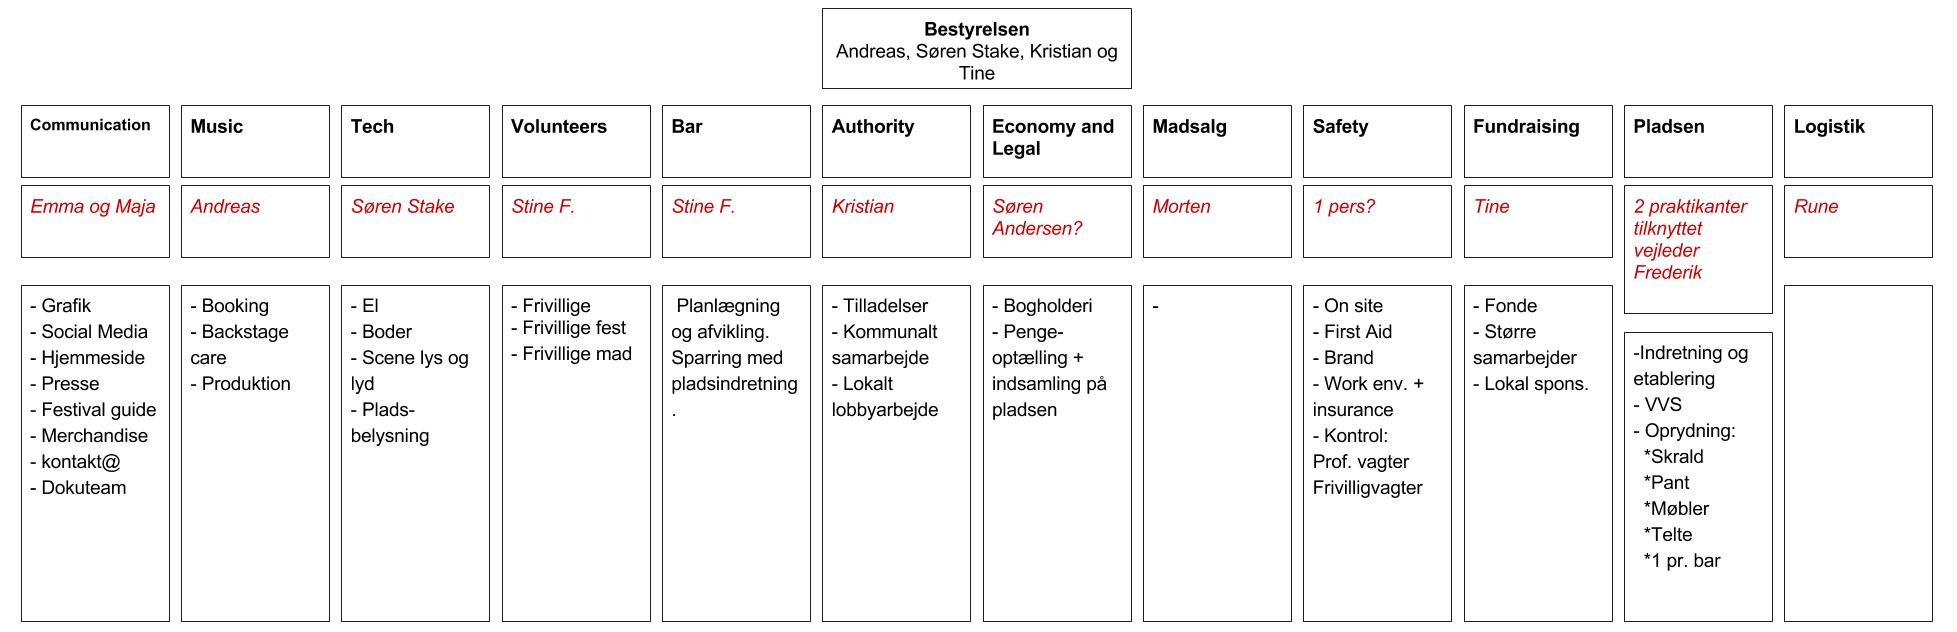
\includegraphics[scale=0.3, angle=90]{Pictures/MIL_Organisational_chart-Ledelsen.jpg}
\section{Business and IT scope}
For this project the workgroup have chosen to focus on the managing part and more specific the board of Musik I lejet. We will also look at how the internal communication is shared between all members and what kind of work processes is in play when planning the festival. \\
Must of the communication is done at Musik i Lejet's Podio site and therefore we will direct our attention and observations towards that platform. Since this projects is done before the actual festival takes place, we will primarily focus on IT used before the festival, which to our belief, is only Podio.  
